\uuid{ReNe}
\chapitre{Autre}
\niveau{L3}
\module{Topologie}
\sousChapitre{Autre}
\titre{OPTRN}
\theme{réseaux de neurones}
\auteur{Quentin Liard}
\datecreate{2024-10-11}
\organisation{AMSCC}
\difficulte{2}
\contenu{
	\texte{
		Soit le réseau de neurones multicouches décrit par le graphe suivant :
		
		\begin{center}
			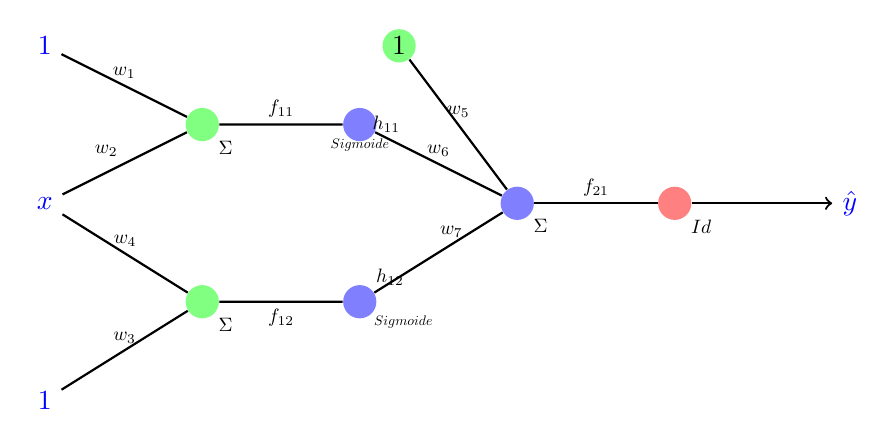
\begin{tikzpicture}[scale=1]
				\def\layersep{2cm}
				\tikzstyle{every pin edge}=[thick]
				\tikzstyle{neuron}=[circle,fill=black!25,minimum size=12pt,inner sep=0pt]
				\tikzstyle{entree}=[];
				\tikzstyle{input neuron}=[neuron, fill=green!50];
				\tikzstyle{output neuron}=[neuron, fill=red!50];
				\tikzstyle{hidden neuron}=[neuron, fill=blue!50];
				\tikzstyle{annot} = [text width=4em, text centered]
				
				% Entree
				\node[entree,blue] (E-1) at (-\layersep,-0.5) {$1$};
				\node[entree,blue] (E-2) at (-\layersep,-2.5) {$x$};
				\node[entree,blue] (E-3) at (-\layersep,-5) {$1$};
				
				% Premiere couche
				\node[input neuron] (I-1) at (0,-1.5) {};
				\node[input neuron] (I-3) at (0,-3.75) {};
				
				\node[below right=0.8ex,scale=0.7] at (I-1) {$\Sigma$};
				\node[below right=0.8ex,scale=0.7] at (I-3) {$\Sigma$};
				
				%Seconde couche et sortie
				\node[hidden neuron] (O) at (\layersep,-3.75 cm) {};
				\node[hidden neuron] (P) at (\layersep,-1.5 cm) {};
				\node[above right=0.8ex,scale=0.7] at (O) {$h_{12}$};
				\node[right=0.5ex,scale=0.7] at (P) {$h_{11}$};
				
				% Arrete et poids
				\path[thick] (E-1) edge node[pos=0.5,above,scale=0.7]{$w_{1}$} (I-1) ;
				\path[thick] (E-2) edge node[pos=0.5,above left,scale=0.7]{$w_{2}$} (I-1);
				\path[thick] (E-2) edge node[pos=0.5,above,scale=0.7]{$w_4$} (I-3);
				\path[thick] (E-3) edge node[pos=0.5,above,scale=0.7]{$w_3$} (I-3);
				\path[thick] (I-1) edge node[pos=0.5,above,scale=0.7]{$f_{11}$} (P);
				\path[thick] (I-3) edge node[pos=0.5,below,scale=0.7]{$f_{12}$}(O);
				\node[below right=0.8ex,scale=0.5] at (O) {$\text{Sigmoide}$};
				\node[below =0.8ex,scale=0.5] at (P) {$\text{Sigmoide}$};
				
				%3eme couche et sortie
				\node[hidden neuron] (Q) at (2*\layersep,-2.5 cm) {};
				\node[output neuron] (R) at (3*\layersep,-2.5 cm) {};
				\node[below right=0.8ex,scale=0.7] at (R) {$\text{Id}$};
				\node[input neuron] (I-4) at (2.5,-0.5) {$1$};
				\path[thick] (O) edge node[pos=0.6,above,scale=0.7]{$w_{7}$} (Q) ;
				\node[below right=0.8ex,scale=0.7] at (Q) {$\Sigma$};
				\path[thick] (I-4) edge node[pos=0.5,above,scale=0.7]{$w_{5}$} (Q) ;
				\path[thick] (Q) edge node[pos=0.5,above,scale=0.7]{$f_{21}$} (R);
				\path[thick] (P) edge node[pos=0.5,above,scale=0.7]{$w_{6}$} (Q) ;
				
				\draw[->,thick] (R)-- ++(2,0) node[right,blue]{$\hat{y}$};
				
			\end{tikzpicture}  
		\end{center}
	}
	\begin{enumerate}
		\item \question{ Donner les formules qui déterminent les sorties intermédiaires $f_{11},\,f_{12},\,h_{11},\,h_{12}$ et $f_{21}$ ainsi que la sortie finale $\hat{y}$. }
		\reponse{
			D'après le graphe, les nœuds marqués "1" correspondent aux biais ($w_1, w_3, w_5$). Les équations de propagation avant (forward pass) sont :
			\begin{align*}
				f_{11} &= w_1 + w_2 x \\
				f_{12} &= w_3 + w_4 x \\
				h_{11} &= \sigma(f_{11}) = \frac{1}{1 + e^{-f_{11}}} \\
				h_{12} &= \sigma(f_{12}) = \frac{1}{1 + e^{-f_{12}}} \\
				\hat{y} &= f_{21} = w_5 + w_6 h_{11} + w_7 h_{12}
			\end{align*}
		}
		
		\item \question{ On pose la fonction d'erreur $E(w)=(y-\hat{y})^2.$ En appliquant l'algorithme de backpropagation (méthode de rétropropagation du gradient appliqué au réseau de neurones), déterminer les dérivées partielles $\frac{\partial E(w)}{\partial w_j}$ puis $\frac{\partial \hat{y}}{\partial w_j}$. En déduire les expressions des mises à jour des paramètres $\Delta w_j$ (variation des poids) pour $j=1,\cdots{},7$. }
		\reponse{
			Pour appliquer la backpropagation, on utilise la règle de la chaîne en définissant des termes d'erreur locaux $\delta$.
			La fonction d’erreur est $E = (y - \hat{y})^2$.
			La mise à jour d'un poids $w_j$ avec un pas d'apprentissage $\eta$ est donnée par :
			\[ \Delta w_j = - \eta \frac{\partial E}{\partial w_j} \]
			
			\textbf{Étape 1 : Couche de sortie}
			Calculons le gradient local en sortie $\delta_{out}$ (dérivée de l'erreur par rapport à l'activation linéaire de sortie $f_{21}$) :
			\[
			\delta_{out} = \frac{\partial E}{\partial \hat{y}} \cdot \frac{\partial \hat{y}}{\partial f_{21}} = -2(y - \hat{y}) \cdot 1 = -2(y - \hat{y})
			\]
			On en déduit les dérivées pour les poids de la dernière couche :
			\begin{align*}
				\frac{\partial E}{\partial w_5} &= \delta_{out} \cdot 1  & \implies \frac{\partial \hat{y}}{\partial w_5} = 1 \\
				\frac{\partial E}{\partial w_6} &= \delta_{out} \cdot h_{11} & \implies \frac{\partial \hat{y}}{\partial w_6} = h_{11} \\
				\frac{\partial E}{\partial w_7} &= \delta_{out} \cdot h_{12} & \implies \frac{\partial \hat{y}}{\partial w_7} = h_{12}
			\end{align*}
			
			\textbf{Étape 2 : Couche cachée (Rétropropagation)}
			On propage l'erreur $\delta_{out}$ vers l'arrière via les poids $w_6$ et $w_7$ pour obtenir les erreurs locales des neurones cachés. On note $\sigma'(z) = \sigma(z)(1-\sigma(z))$.
			
			Pour la branche du haut ($h_{11}$) :
			\[ \delta_{h1} = \underbrace{\delta_{out} \cdot w_6}_{\text{Rétropropagation}} \cdot \underbrace{\sigma'(f_{11})}_{\text{Dérivée activation}} = -2(y-\hat{y}) w_6 h_{11}(1-h_{11}) \]
			D'où les dérivées pour $w_1$ et $w_2$ :
			\begin{align*}
				\frac{\partial E}{\partial w_1} &= \delta_{h1} \cdot 1 \implies \frac{\partial \hat{y}}{\partial w_1} = w_6 h_{11}(1-h_{11}) \\
				\frac{\partial E}{\partial w_2} &= \delta_{h1} \cdot x \implies \frac{\partial \hat{y}}{\partial w_2} = w_6 h_{11}(1-h_{11})x
			\end{align*}
			
			Pour la branche du bas ($h_{12}$) :
			\[ \delta_{h2} = \delta_{out} \cdot w_7 \cdot \sigma'(f_{12}) = -2(y-\hat{y}) w_7 h_{12}(1-h_{12}) \]
			D'où les dérivées pour $w_3$ et $w_4$ :
			\begin{align*}
				\frac{\partial E}{\partial w_3} &= \delta_{h2} \cdot 1 \implies \frac{\partial \hat{y}}{\partial w_3} = w_7 h_{12}(1-h_{12}) \\
				\frac{\partial E}{\partial w_4} &= \delta_{h2} \cdot x \implies \frac{\partial \hat{y}}{\partial w_4} = w_7 h_{12}(1-h_{12})x
			\end{align*}
			
			\textbf{Résumé des mises à jour $\Delta w_j = - \eta \frac{\partial E}{\partial w_j}$ :}
			\[
			\Delta w_j = 2\eta(y-\hat{y}) \times \frac{\partial \hat{y}}{\partial w_j}
			\]
			(en remplaçant $\frac{\partial \hat{y}}{\partial w_j}$ par les expressions calculées ci-dessus).
		}
	\end{enumerate}
}